\subsection{Objective}
The purpose of this application is to provide an intuitive as well as interactive tool to visualise transformations and their respective effect on the relation to fixed points in three-dimensional space. 

This tool is supposed to support the development of better test cases as well as aid students in the understanding of trigonometry. This tool is mainly aimed at software testers, as it helps them to get a more tangible vision of possible szenarios and now imaginable edge-cases. A secondary target group are (engineering-)students struggeling to get their head around trigonometry.

Since rotations in space become far more difficult to envision if we are concerned about an arbitrary point on the plane, and its relation to fixed points in space, instead of its center, this issue is being addressed by this application.

Although there are many other rotation visualisation tools out there, none of them visualize the relation to fixed points in space, let you move said points or the plane in space and don’t address afroementioned issues.

\newpage
\subsection{Requirements Refinement}
Previous rough user stories now get a clear testable statement assigned to them. 

Requirements that are tagged with \tcbox[colframe=TAGred, colback=TAGred]{\textbf{\footnotesize \acs{M2FR}}}, could not be implemented in time for the planned release and had to be moved to a future release. \newline Since these requirements are not essential for the core functionality and a timely release is ranked higher than the fulfillment of optional requirements, this was considered justified.


\subsubsection{Functional}
\input{generatedTables/Refined-Requirements-F}

%\subsubsection{Functional - Technical}
% \textbf{TODO:!!!}
%Requirements for more technical aspects of the application that are not facing the user directly.
%
    \bgroup
    \def\arraystretch{1.5}
    \setlength\arrayrulewidth{1.2pt}
    \color{textgray}
    \begin{xltabular}{\textwidth}{|X|M{1.5cm}|M{1.5cm}|}

\caption*{} \label{tab:Requirements - Functional Technical} \\

\arrayrulecolor{linegray}\hline \rowcolor{lightgray} \multicolumn{1}{|c|}{\color{default}\textbf{Requirement}} & \multicolumn{1}{c|}{\color{default}\textbf{Jira Issue}} & \multicolumn{1}{c|}{\color{default}\textbf{Status}}\\ \hline

 \endfirsthead 
 \multicolumn{3}{c}%
{\tablename\ \thetable{} -- continued from previous page} \\ \hline \multicolumn{1}{|c|}{\textbf{Requirement}} & \multicolumn{1}{c|}{\textbf{Jira Issue}} & \multicolumn{1}{c|}{\textbf{Status}}\\ \hline 
\endhead \hline 
\multicolumn{3}{|r|}{{Continued on next page}} \\ \hline 
\endfoot

\hline 
 \endlastfoot 
azimuthAngle & {\color{purpleT}\ttfamily TECH-001} & \tcbox[colframe=TAGgreen, colback=TAGgreen]{\textbf{\footnotesize DONE}} \\ \hline 
  
\end{xltabular} 
 \egroup 
 \color{default}

\subsubsection{Non-Functional}

    \bgroup
    \def\arraystretch{1.5}
    \setlength\arrayrulewidth{1.2pt}
    \color{textgray}
    \begin{xltabular}{\textwidth}{|X|M{2cm}|M{2cm}|}

\caption*{} \label{tab:Requirements - Functional Technical} \\

\arrayrulecolor{linegray}\hline \rowcolor{lightgray} \multicolumn{1}{|c|}{\color{default}\textbf{Requirement}} & \multicolumn{1}{c|}{\color{default}\textbf{Importance}} & \multicolumn{1}{c|}{\color{default}\textbf{Status}}\\ \hline

 \endfirsthead 
 \multicolumn{3}{c}%
{\tablename\ \thetable{} -- continued from previous page} \\ \hline \multicolumn{1}{|c|}{\textbf{Requirement}} & \multicolumn{1}{c|}{\textbf{Importance}} & \multicolumn{1}{c|}{\textbf{Status}}\\ \hline 
\endhead \hline 
\multicolumn{3}{|r|}{{Continued on next page}} \\ \hline 
\endfoot

\hline 
 \endlastfoot 
The Application shall run smoothly in the following browsers:\newline  Chrome $\ge$ 109\newline \newline FireFox $\ge$ 98\newline  \newline  Opera $\ge$ 100 & \tcbox[colframe=TAGred, colback=TAGred]{\textbf{\footnotesize HIGH}} & \tcbox[colframe=TAGgreen, colback=TAGgreen]{\textbf{\footnotesize DONE}} \\ \hline 
  Images shall either have the format .svg or .webp. & \tcbox[colframe=TAGyellow, colback=TAGyellow]{\textbf{\footnotesize MEDIUM}} & \tcbox[colframe=TAGgreen, colback=TAGgreen]{\textbf{\footnotesize DONE}} \\ \hline 
  The application shall run as a dockersied container. & \tcbox[colframe=TAGred, colback=TAGred]{\textbf{\footnotesize HIGH}} & \tcbox[colframe=TAGyellow, colback=TAGyellow]{\textbf{\footnotesize PENDING}} \\ \hline 
  An instance of the project shall be directly accessible via the internet. & \tcbox[colframe=TAGred, colback=TAGred]{\textbf{\footnotesize HIGH}} & \tcbox[colframe=TAGyellow, colback=TAGyellow]{\textbf{\footnotesize PENDING}} \\ \hline 
  
\end{xltabular} 
 \egroup 
 \color{default}

\newpage
\subsection{Out of Scope}
\begin{itemize}
\item \textbf{Possibility for the user to enter a full transformation matrix by hand.}
\item \textbf{Adding a Trajectories} - via speed vectors in x,y and z direction. And calculating possible intersections/collisions.
\item \textbf{Mobile responsiveness} - mobile users aren't the target audience. Therefore the extra time can not be justified.
\item \textbf{A complete automated Frontend Test Suite} - currently I confined myself to manual tests after every major update to ensure correct functionality. This is feasible since the scope/functionality of this project is comparably small and the extra time can not be justified.
\item \textbf{Backwards compatibility with older browser}
\item \textbf{Assure correct rendering in more niche browsers}
\item \textbf{Undo/Redo functionality}
\item \textbf{Add a 2D (\enquote{Ship}-)Mode} - Still render everything in 3D but give the option to be limited to the ground and render the plane as a ship. In this case threats could come from above and below.
\item \textbf{Move and rotate Marble arbitrarily} - The point on the plane from which all measurements are calculated shall be freely positionable in relation to the plane.
\end{itemize}

\subsection{Requirements that were moved to the next release.}

These requirements were not fulfillable in the set time frame and had to be moved to the next release since they are not vital for the intended functionality of the app.

\begin{itemize}
\item {\textbf{\color{TAGpurple}\ttfamily DLMCSPSE-238 }}(Math Explanation Page)
\item {\textbf{\color{TAGpurple}\ttfamily DLMCSPSE-237 }}(Math Explanation Page)
\item {\textbf{\color{TAGpurple}\ttfamily DLMCSPSE-243 }}(404 Page)
\end{itemize}

\newpage
\subsection{Documentation of Software \& System Architecture}

The basic architecture of this web-application follows the schematic sketched in Figure \ref{fig:flow_chart}.

\begin{figure}[!h]
  \centering
  \caption{Basic structure of the web application}
  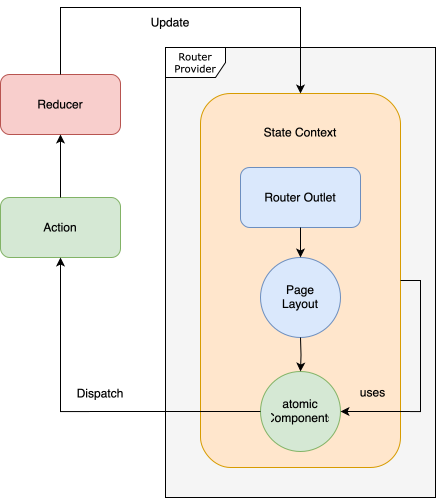
\includegraphics[width=\textwidth]{assets/Flow-Diagram.png}
  \label{fig:flow_chart}
\end{figure}

\newpage

Pages (rectangles) and Components (circles) that are involved in updating and consuming the state context are presented in Figure  \ref{fig:uml_diagram}.

\begin{figure}[!h]
  \centering
  \caption{Flow of Components involved in updating and consuming the state context}
  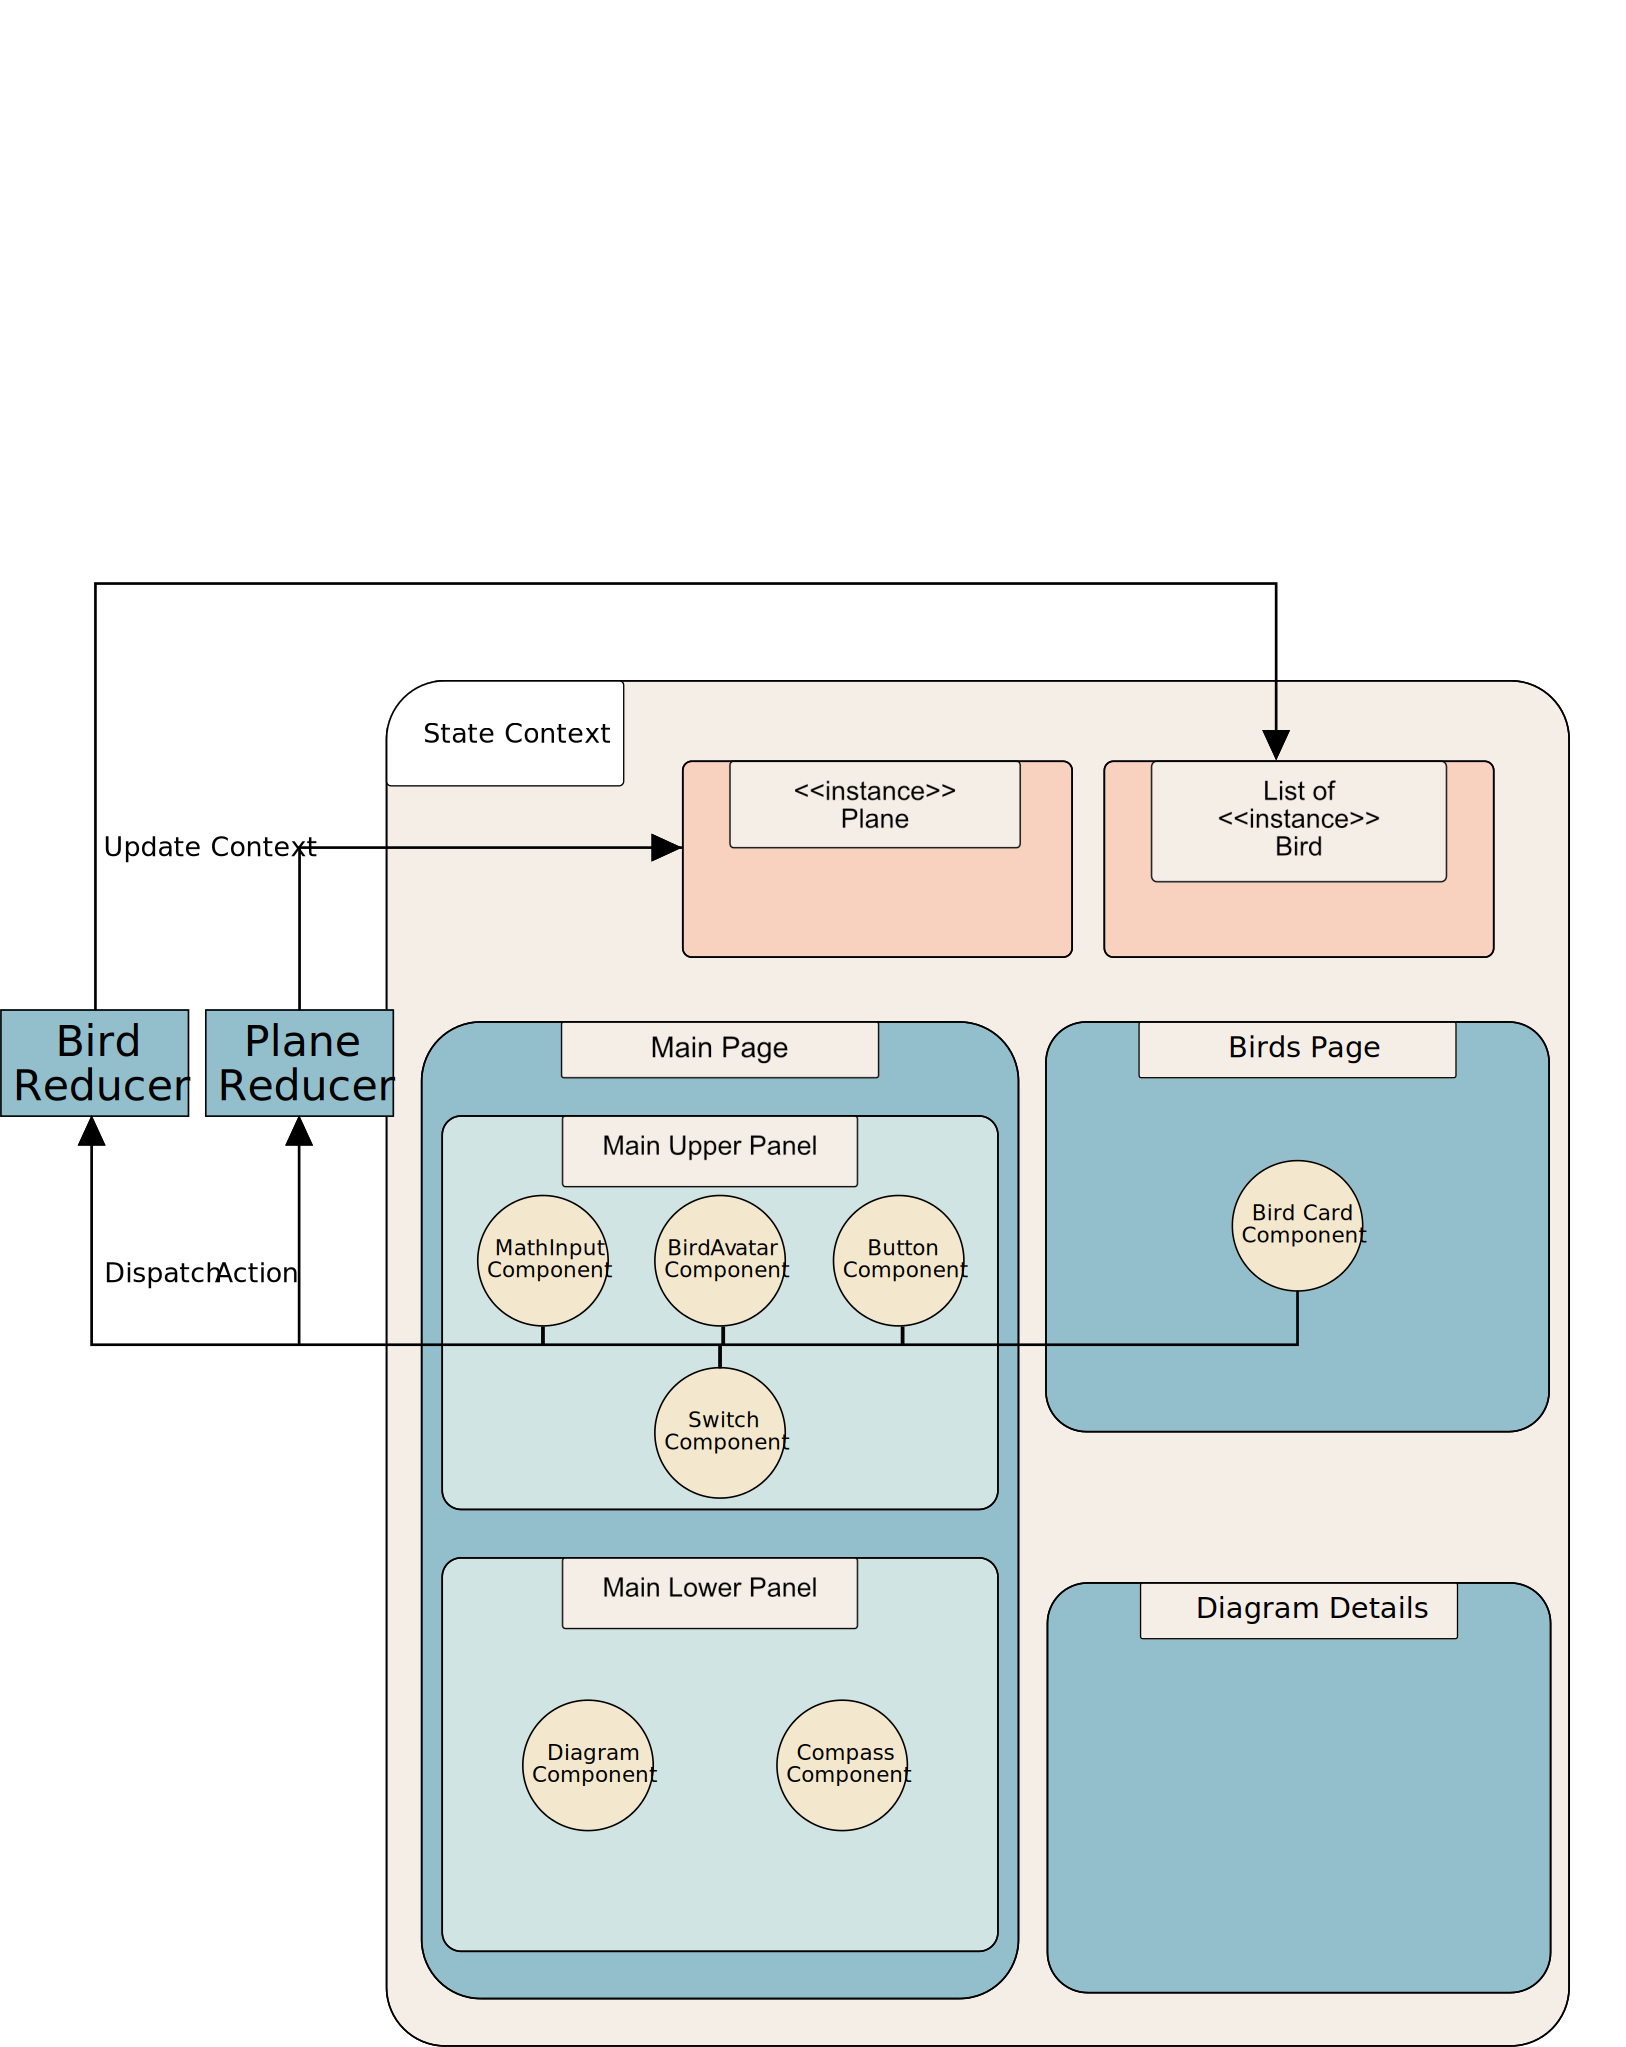
\includegraphics[width=\textwidth]{assets/uml_diagram.png}
  \label{fig:uml_diagram}
\end{figure}

\newpage
\subsection{Design and Implementation Procedure}
The design process was mostly defined by drawing and redefining new mock-ups that were refined after each sprint. The implementation of mathematical functions followed a \ac{TDD} procedure.

\subsection{Used 3rd Party Libraries}
The following 3rd party libraries were finally used in the making of this application. 
\begin{itemize}
  \item React (\cite{React})
  \item React Router (\cite{ReactRouter})
  \item React Icons (\cite{ReactIcons})
  \item Chakra-UI (\cite{chakra})
  \item PlotlyJS (\cite{PlotlyJS})
  \item Vite (\cite{Vite})
  \item Vitest (\cite{Vitest})
  \item Docker (\cite{Docker})
\end{itemize}